\section{Detailed Proofs}

\subsection{Proof of Theorem~\ref{lemma:non-realisable}}\label{sec:proof_non_realisability}
\begin{proof}[Proof of Theorem~\ref{lemma:non-realisable}]
We begin by introducing the appropriate definitions and lemmas.  

\begin{definition}[$\epsilon$-homogeneity]\label{def:eps_homo}
    Given two MDPs $\mdp_1 = (\mathcal{S}, \mathcal{A}, \mathcal{R}, \mathcal{T}_1, \gamma)$ and $\mdp_2 = (\mathcal{S}, \mathcal{A}, \mathcal{R}, \mathcal{T}_2, \gamma)$ we say $\mdp_2$ is a $\epsilon$-homogenous partition of $\mdp_1$ with respect to $L_k$ norm if
    \begin{equation}
        \forall a \in \mathcal{A} \quad \Big(\sum_{s' \in \mathcal{S}} \big(\sum_{s\in\mathcal{S}}\mathcal{T}_1(s, a, s')-\mathcal{T}_2(s, a, s')\big)^k\Big)^{\frac{1}{k}} \leq \epsilon.
    \end{equation}
\end{definition}

Note that this definition of $\epsilon$-homogeneity is a special case of Definition 3~\citep{even2003approximate}, where the reward functions and state spaces are taken to be identical. We will only study partitions with respect to the $L_1$ norm between transition probabilities.

\begin{lemma}[Lemma 3~\citep{even2003approximate}]\label{lemma:same_pol}
    Let $\mdp_2$ be an $\epsilon$-homogenous partition of $\mdp_1$, then, with respect to $L_1$ norm, an arbitrary policy $\pol$ in $\mdp_2$ induces an $\frac{\epsilon}{(1-\gamma)^2}-$optimal policy in $\mdp_1$.
    \begin{equation}
        ||V_{\mdp_1}^\pol-V_{\mdp_2}^\pol||_\infty \leq \frac{\epsilon}{(1-\gamma)^2}.
    \end{equation}
    %This is shown in~\citep{even2003approximate} using the following argument,
    %\begin{equation}
     %   \underset{s\in\mathcal{S}}{\max} \, |V_{\mdp_1}^\pol-V_{\mdp_2}^\pol| = ||V_0^\pol-V_{\mdp_1}^\pol||\infty = ||V_0^\pol-V_\infty^\pol||_\infty \leq \frac{\epsilon}{(1-\gamma)^2},
    %\end{equation}
    %where $V_\infty^\pol = V_{\mdp_1}^\pol$ is the value of $\pol$ in $\mdp_1$.
\end{lemma}

\begin{lemma}[Lemma 4~\citep{even2003approximate}]\label{lemma:opt_opt}
    Let $\mdp_2$ be an $\epsilon$-homogenous partition of $\mdp_1$, then, with respect to $L_1$ norm, the optimal policy in $\mdp_2$ induces an $\frac{2\epsilon}{(1-\gamma)^2}-$optimal policy in $\mdp_1$. 
    \begin{equation}
        ||V_{\mdp_1}^*-V_{\mdp_2}^*||_\infty \leq \frac{2\epsilon}{(1-\gamma)^2}.
    \end{equation}
    %This is shown in~\citep{even2003approximate} using the following, by Lemma~\ref{lemma:same_pol},
    %\begin{equation}
     %   \underset{s\in\mathcal{S}}{\max} \, |V_{\mdp_1}^{\pol^{*}(\mdp_2)}(s)-V_{\mdp_1}^{*}(s)| \leq \frac{\epsilon}{(1-\gamma)^2}.
    %\end{equation}
    %Then, if Value Iteration is used on $\mdp_1$ with initial value $V_0^{\mdp_1}(s)=V_{\mdp_2}^{\pol^*(\mdp_1)}(s)$ we have that,
    %\begin{equation}
    %    ||V_0^{\mdp_1}-V_\infty^{\mdp_1}||_\infty=||V_0^{\mdp_1}-V_{\mdp_1}^{*}||_\infty \leq \frac{\epsilon}{(1-\gamma)^2}.
    %\end{equation}
    %If $L_1$ norm is used, then $||V_0^{\mdp_1}-V_1^{\mdp_1}||_\infty \leq \frac{\epsilon}{1-\gamma}$. Combining these leads to that $\pol^*(\mdp_2)$ is an $\frac{2\epsilon}{(1-\gamma)^2}$ policy in $\mdp_1$. 
\end{lemma}

Given the assumptions in Theorem~\ref{lemma:non-realisable} hold true. Then, using the $\epsilon-$homogeneity definition in Definition~\ref{def:eps_homo}, let $\hat{\mdp}$ be an $\epsilon_{\mathrm{Estim}}-$homogenous partition of $\mdp$ and $\mdp$ be an $\epsilon_{\mathrm{Realise}}-$homogenous partition of $\mdp^*$. Under the $L_1$ norm then, we have     
    \begin{align}
        \forall a \in \mathcal{A} \quad &\Big(\sum_{s' \in \mathcal{S}} \sum_{s\in\mathcal{S}}\mathcal{T}(s, a, s')-\hat{\mathcal{T}}(s, a, s')\Big) \leq \epsilon_{\mathrm{Estim}},\\
         &\Big(\sum_{s' \in \mathcal{S}} \sum_{s\in\mathcal{S}}\mathcal{T}^*(s, a, s')-\mathcal{T}(s, a, s')\Big) \leq \epsilon_{\mathrm{Realise}}.
    \end{align}
Using triangle inequalities we can then bound the $L_1$ norm between the true underlying MDP and the maximum likelihood estimator,
\begin{align}
     \forall a \in \mathcal{A} \quad &\Big(\sum_{s' \in \mathcal{S}} \sum_{s\in\mathcal{S}}\mathcal{T}^*(s, a, s')-\hat{\mathcal{T}}(s, a, s')\Big)\\
    = \, &\Big(\sum_{s' \in \mathcal{S}} \sum_{s\in\mathcal{S}}\mathcal{T}^*(s, a, s')-\mathcal{T}(s,a,s')+\mathcal{T}(s,a,s')-\hat{\mathcal{T}}(s, a, s')\Big)\\
    \leq \, &\Big(\sum_{s' \in \mathcal{S}} \sum_{s\in\mathcal{S}}\mathcal{T}^*(s, a, s')-\mathcal{T}(s,a,s')\Big) +\Big(\sum_{s' \in \mathcal{S}} \sum_{s\in\mathcal{S}}\mathcal{T}(s, a, s')-\hat{\mathcal{T}}(s,a,s')\Big)\\ \leq \, &\epsilon_{\mathrm{Estim}}+\epsilon_{\mathrm{Realise}}.
\end{align}

Thus, $\hat{\mdp}$ is a $(\epsilon_{\mathrm{Estim}}+\epsilon_{\mathrm{Realise}})-$homogenous partition of $\mdp^*$. The next steps involves creating a bound on the performance gap between the value functions and policies in $||V_{{\mdp^*}}^{*}-V_{{\mdp^*}}^{\hat{\pol}}||_\infty$. Using triangle inequalities the performance gap can be expanded further,

\begin{equation}
\begin{aligned}\label{eq:triangle}
    ||V_{{\mdp^*}}^{*}-V_{{\mdp^*}}^{\hat{\pol}}||_\infty &= ||V_{{\mdp^*}}^{*}-V_{\hat{\mdp}}^{\hat{\pol}}+V_{\hat{\mdp}}^{\hat{\pol}}-V_{{\mdp^*}}^{\hat{\pol}}||_\infty\\
    &\leq ||V_{{\mdp^*}}^{*}-V_{\hat{\mdp}}^{\hat{\pol}}||_\infty+||V_{\hat{\mdp}}^{\hat{\pol}}-V_{{\mdp^*}}^{\hat{\pol}}||_\infty.
\end{aligned}
\end{equation}

The first term on the right side of the inequality in Eq.~\ref{eq:triangle} can be bounded using Lemma~\ref{lemma:opt_opt} since $\hat{\pol}$ is the optimal policy in $\hat{\mdp}$,

\begin{equation}
    ||V^{*}_{\mdp^{*}}-V_{\hat{\mdp}}^{\hat{\pol}}||_\infty \leq \frac{2(\epsilon_{\mathrm{Estim}}+\epsilon_{\mathrm{Realise}})}{(1-\gamma)^2}.
\end{equation}
Likewise, the second term in the inequality can be bounded using Lemma~\ref{lemma:same_pol},

\begin{equation}
    ||V_{\hat{\mdp}}^{\hat{\pol}}-V_{\mdp^*}^{\hat{\pol}}||_\infty \leq \frac{\epsilon_{\mathrm{Estim}}+\epsilon_{\mathrm{Realise}}}{(1-\gamma)^2}.
\end{equation}

Combining these two terms yields us $||V_{{\mdp^*}}^{*}-V_{{\mdp^*}}^{\hat{\pol}}||_\infty \leq \frac{3(\epsilon_{\mathrm{Estim}}+\epsilon_{\mathrm{Realise}})}{(1-\gamma)^2}$.
%Finally, the rightmost term in Eq.~\ref{eq:non-realisable-triplet} can be bounded using Theorem 6.5.9~\citep{dimitrakakis2018decision}.
%\begin{equation}\label{eq:value_iteration}
%    |V_{{\mdp^*}}^{\hat{\pol}}-\hat{V}_{{\mdp^*}, t}^{\hat{\pol}}| \leq \frac{2\gamma^t}{1-\gamma}.
%\end{equation}
%Finally, joining Eq.~\ref{eq:bias_bound} and Eq.~\ref{eq:value_iteration} yields us the result.
\end{proof}

\subsection{Proof of Remark~\ref{remark:l1_norm}}\label{sec:proof_remark}
\begin{proof}[Proof of Remark~\ref{remark:l1_norm}]
    The analysis of the concentration of $\epsilon_{\mathrm{Estim}}$ follows the works of~\citep{auer2008near, qian2020concentration}. Let $\Delta^{\mathcal{S}}$ be the $(\mathcal{S}-1)-$dimensional simplex and $\mathcal{T}_{s,a}^* \in \Delta^{\mathcal{S}}$ be the transition kernel for a state-action pair of the true underlying MDP $\mu^*$ and $\hat{\mathcal{T}}_{s,a} \in \Delta^{\mathcal{S}}$ a random vector. If $\hat{\mathcal{T}}_{s,a}$ is taken to be the empirical estimate of $\mathcal{T}_{s,a}^*$ then the following lemma can be invoked.
    
    \begin{proposition}[\citep{weissman2003inequalities}]\label{lemma:weissman}
        Let $\mathcal{T}_{s,a}^* \in \Delta^{\mathcal{S}}$ and $\hat{\mathcal{T}}_{s,a} \sim \frac{1}{n^{s,a}}\mathrm{Multinomial}(n^{s,a}, \mathcal{T}_{s,a}^*)$. Then, for $S \geq 2, \delta \in [0, 1]$ and $n^{s,a} \geq 1$,
        \begin{align}
            &\mathbb{P}\Bigg(||\mathcal{T}_{s,a}^*-\hat{\mathcal{T}}_{s,a}||_1\geq \sqrt{\frac{2S\log(2/\delta)}{n^{s,a}}}\Bigg) \notag\\
            \leq &\mathbb{P}\Bigg(||\mathcal{T}_{s,a}^*-\hat{\mathcal{T}}_{s,a}||_1 \geq \sqrt{\frac{2\log\big((2^S -2)/\delta)\big)}{n^{s,a}}}\Bigg)\leq \delta.
        \end{align}
    \end{proposition}
    The invocation of Proposition~\ref{lemma:weissman}, with $T=\sum_{s\in\mathcal{S}}\sum_{a\in\mathcal{A}}n^{s,a}$ yields us a $L_1$ norm bound for the difference of transition kernels associated with a particular state-action pair $s, a$. Next, union bounding over all possible state and action combinations yields us a bound on the total $L_1$ norm.
    \begin{align}
        &\mathbb{P}\Bigg(\bigcup_{s\in\mathcal{S}}\bigcup_{a\in\mathcal{A}}\Big(||\mathcal{T}_{s,a}^*-\hat{\mathcal{T}}_{s,a}||_1\geq \sqrt{\frac{2\log\big((2^S -2)/\delta)\big)}{n^{s,a}}}\Big)\Bigg)\\
        \leq &\sum_{s\in\mathcal{S}}\sum_{a\in\mathcal{A}} \mathbb{P}\Bigg(||\mathcal{T}_{s,a}^*-\hat{\mathcal{T}}_{s,a}||_1\geq \sqrt{\frac{2\log\big((2^S -2)/\delta)\big)}{n^{s,a}}}\Bigg)\\
        \leq &SA\delta.
    \end{align}
    From this, we have that, with probability $1-SA\delta$,
    \begin{equation}
        ||\mathcal{T}^*-\hat{\mathcal{T}}||_1 \leq \epsilon_{\mathrm{Estim}} \leq \sum_{s\in\mathcal{S}}\sum_{a\in\mathcal{A}}\sqrt{\frac{2\log\big((2^S -2)/\delta)\big)}{n^{s,a}}}.
    \end{equation}
    The total $L_1$ norm then scales on the order of $\mathcal{O}(SA\sqrt{S-\log(\delta)}/\sqrt{T})$, which is the final result.
\end{proof}

%\clearpage
\section{Details of Planning: \textsc{RiccatiIteration}}\label{sec:riccati}
An LQR-based control system is defined by its system matrices~\citep{kalman1960new}. Let $d_s$ be the state dimensionality and $d_a$ be the action dimensionality. Then, $\mathbf{A} \in \mathbb{R}^{d_s}\times\mathbb{R}^{d_s}$ is a matrix describing state associated state transitions. $\mathbf{B} \in \mathbb{R}^{d_s}\times\mathbb{R}^{d_a}$ is a matrix describing control associated state transitions. The final two system matrices are cost related with $\mathbf{Q} \in \mathbb{R}^{d_s}\times\mathbb{R}^{d_s}$ being a positive definite cost matrix of states and $\mathbf{R} \in \mathbb{R}^{d_a}\times\mathbb{R}^{d_a}$ a positive definite cost matrix of control inputs. The transition model described under this model is given by,
\begin{equation}
   \bm{s}_{t+1}-\bm{s}_t = \mathbf{A}\bm{s}_t + \mathbf{B}\bm{a}_t.
\end{equation}

When an MDP is mentioned in the context of an LQR system in this work, the MDP is the set of system matrices. Further, the cost (or reward) of a policy $\pol$ under an MDP $\mdp$ is
\begin{equation}
    V_{\mdp}^\pol = \sum_{t=0}^T \bm{s}_t^\top \mathbf{Q}\bm{s}_t + \bm{a}_t^\top \mathbf{R}\bm{a}_t.
\end{equation}
Optimal policy identification can be accomplished using~\citep{willems1971least}. It begins by solving for the cost-to-go matrix $\mathbf{P}$ by,
\begin{align*}
   \underset{\mathbf{P}}{\textrm{solve}}~~~~\mathbf{A}^\top \mathbf{P}\mathbf{A}-\mathbf{P}+\mathbf{Q}-(\mathbf{A}^\top \mathbf{P}\mathbf{B})(\mathbf{R}+\mathbf{B}^\top\mathbf{P}\mathbf{B})^{-1}(\mathbf{B}^\top \mathbf{P}\mathbf{A}) = 0.
\end{align*}

Then, using $\mathbf{P}$ the control input $\bm{a}$ for a particular state $\bm{s}$ is
\begin{equation}
   \bm{a} = -(\mathbf{R}+\mathbf{B}^\top\mathbf{P}\mathbf{B})^{-1}(\mathbf{B}^\top\mathbf{P}\mathbf{A})\bm{s}.
\end{equation}

With some abuse of notation and for compactness, we allow ourselves to write $\bm{a}_t = -(\mathbf{R}+\mathbf{B}^\top\mathbf{P}\mathbf{B})^{-1}(\mathbf{B}^\top\mathbf{P}\mathbf{A})\bm{s}_t$ for $\bm{a}_t \sim \pol(\bm{s}_t)$.

% \section{Meta-Algorithm for MLEMTRL in the Non-Realisable Setting}\label{sec:meta_mlemtrl}

% In order to guarantee good performance even in the non-realisable setting one might think of adding the target task to the set of source tasks or constructing a meta-algorithm, combining the model estimated by MLEMTRL and the empirical estimation of the target task. In this section we propose a meta-algorithm based on the latter, in Algorithm~\ref{alg:meta-mlemtrl}. The main change in the algorithm is internally keeping track of the empirical model and on Line~\ref{lin:meta-mlemtrl}, computing a posterior probability distribution over the respective models by weighting the two likelihoods together with their respective priors. How much the meta-algorithm should focus on the empirical model is then decided by the prior, because $\ell_{\mathrm{Empirical}} \geq \ell_{\mathrm{MLEM}}$. For experimental results using this algorithm, see Figure~\ref{fig:meta_results}.

% \begin{algorithm}[ht!]
% \caption{Meta-MLEMTRL}\label{alg:meta-mlemtrl}
% \begin{algorithmic}[1]
% %\STATE ${\textsc{MLEMTRL}(\bm{w}^0,\mathcal{M}_s, D_0, \lambda, \gamma, T}) $
% \STATE \textbf{Input:} prior $p$, weights $\bm{w}^0$, $m$ source MDPs $\mathcal{M}_s$, data $D_0$, discount factor $\gamma$, iterations $T$.
% \FOR{$t=0, \hdots, T$}
% \STATE\textsc{// Stage 1: Obtain Model Weights //}
% %\STATE \hspace{1.0cm} $\bm{w}^{t+1}\leftarrow  \bm{w}^t -\lambda\nabla_{\bm{w}}\log\mathbb{P}(D_t \, | \, \Sigma_{i=1}^m w_i \mdp_i), D_t \sim \mdp^{*}, \mdp_i\in\mathcal{M}_s$
% \STATE $\bm{w}^{t+1}\leftarrow  \textsc{MLEMTRL}(\bm{w}^t, \mathcal{M}_s, \mathcal{D}_t, \gamma, 1)$
% \STATE Estimate the MDP: $\mdp^{t+1} = \sum_{i=1}^m w_i \mdp_i$
% \STATE Compute log-likelihood $\ell_{\mathrm{MLEM}}^{t+1} = \log \mathbb{P}(\mathcal{D}_t \, | \, \mdp^{t+1})$
% \STATE Compute log-likelihood of empirical model  $\ell_{\mathrm{Empirical}}^{t+1} = \log \mathbb{P}(\mathcal{D}_t \, | \, \hat{\mdp}^{t+1})$ 
% %\STATE Compute maximum a posteriori $\tilde{\mdp}^{t+1} = \arg\max \Big\{\mathbb{P}(\mdp^{t+1})=\exp\Big(\ell_{\mathrm{MLEM}}^{t+1}\Big)p, \mathbb{P}(\hat{\mdp}^{t+1})= \exp\Big(\ell_{\mathrm{Empirical}}^{t+1}\Big)(1-p)\Big\}$\label{lin:meta-mlemtrl}
% \STATE Sample $\tilde{\mdp}^{t+1}$ as $\mdp^{t+1}$ w.p. $\propto p\exp\Big(\ell_{\mathrm{MLEM}}^{t+1}\Big)$ and $\hat{\mdp}^{t+1}$ w.p. $\propto (1-p)\exp\Big(\ell_{\mathrm{Empirical}}^{t+1}\Big)$.\label{lin:meta-mlemtrl}
% \STATE\textsc{// Stage 2: Model-based Planning //}
% \STATE Compute the policy: $\pol^{t+1} \in \underset{\pol}{\arg\max} \, V_{\tilde{\mdp}^{t+1}}^\pol$
% \STATE\textsc{// Control //}
% \STATE Observe $s_{t+1}, r_{t+1} \sim \mdp^{*}(s_t, a_t), a_t\sim \pol^{t+1}(s_t)$
% \STATE Update the dataset $D_{t+1} = D_t \cup \{s_t, a_t, s_{t+1}, r_{t+1}\}$
% \ENDFOR
% %\RETURN An estimated MDP model $\tilde{\mdp}^T$ and a policy $\pol^T$
% \STATE \textbf{return} An estimated MDP model $\tilde{\mdp}^T$ and a policy $\pol^T$
% \end{algorithmic}
% \end{algorithm}

% \begin{figure*}[h!]
%     \centering
%     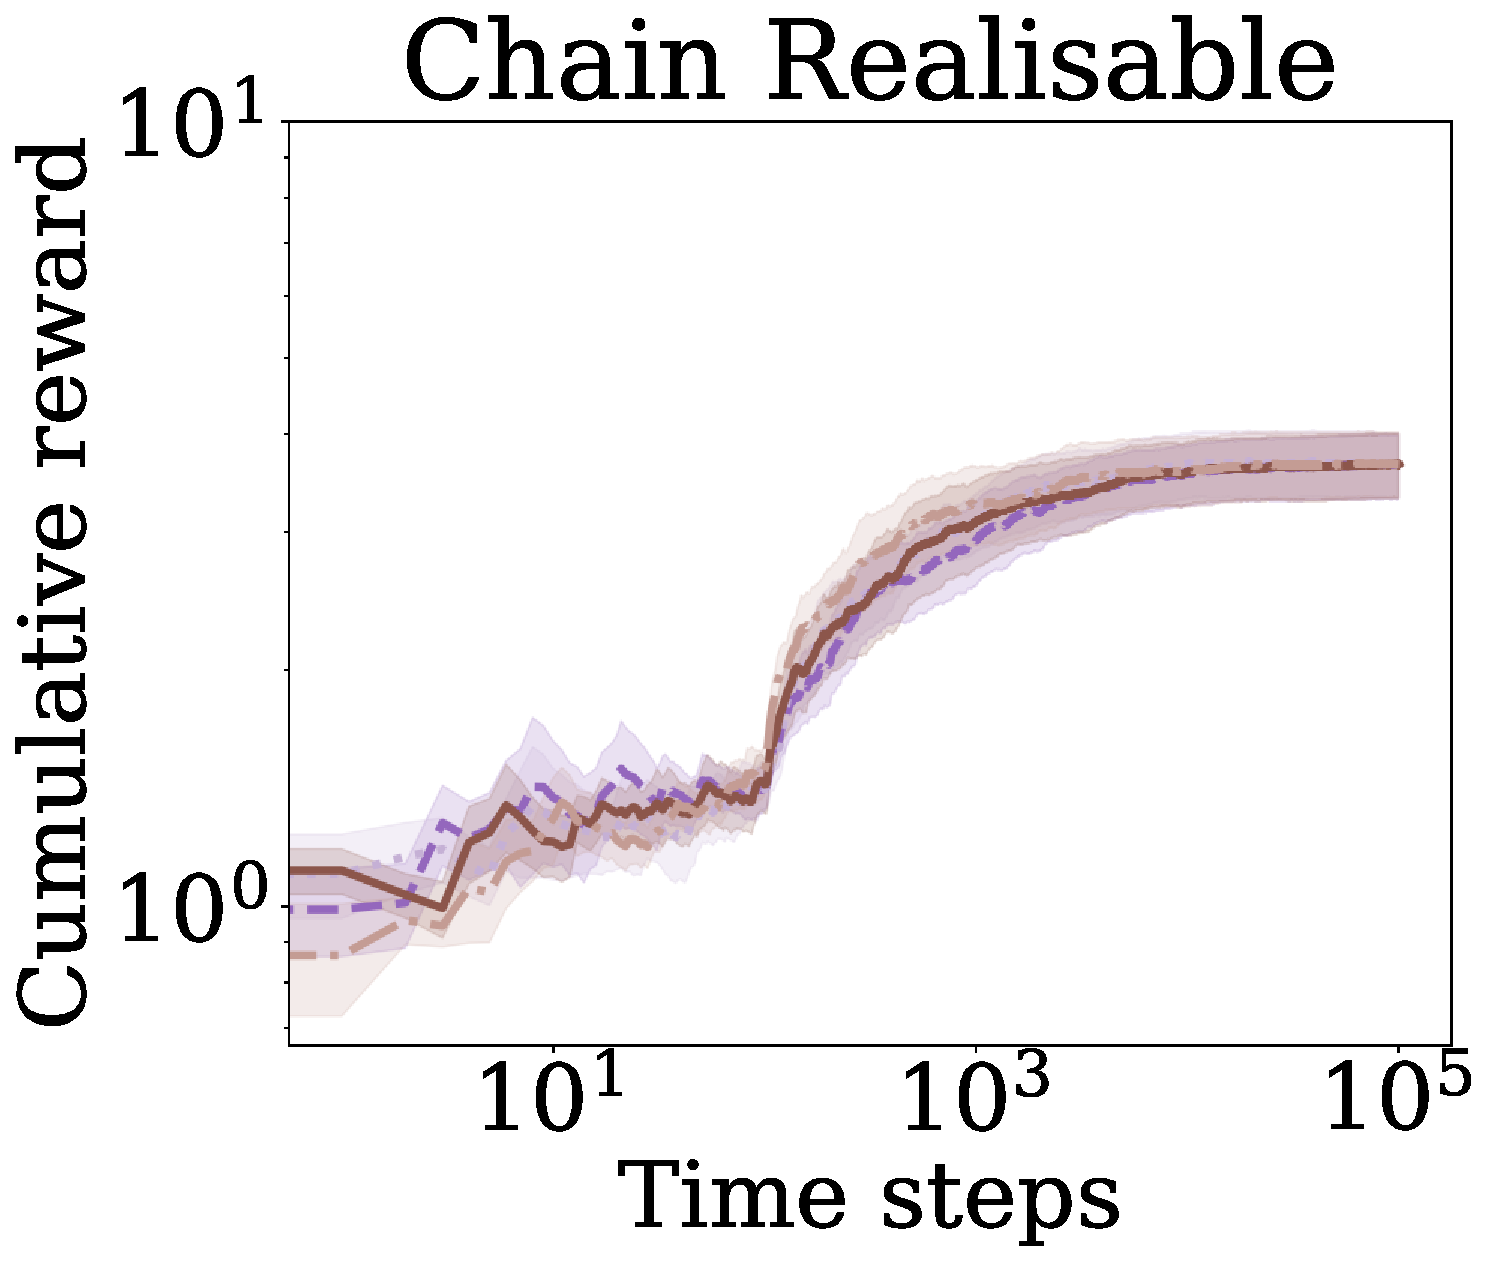
\includegraphics[width=0.35\textwidth]{img/chain_meta_realisable.pdf} 
%     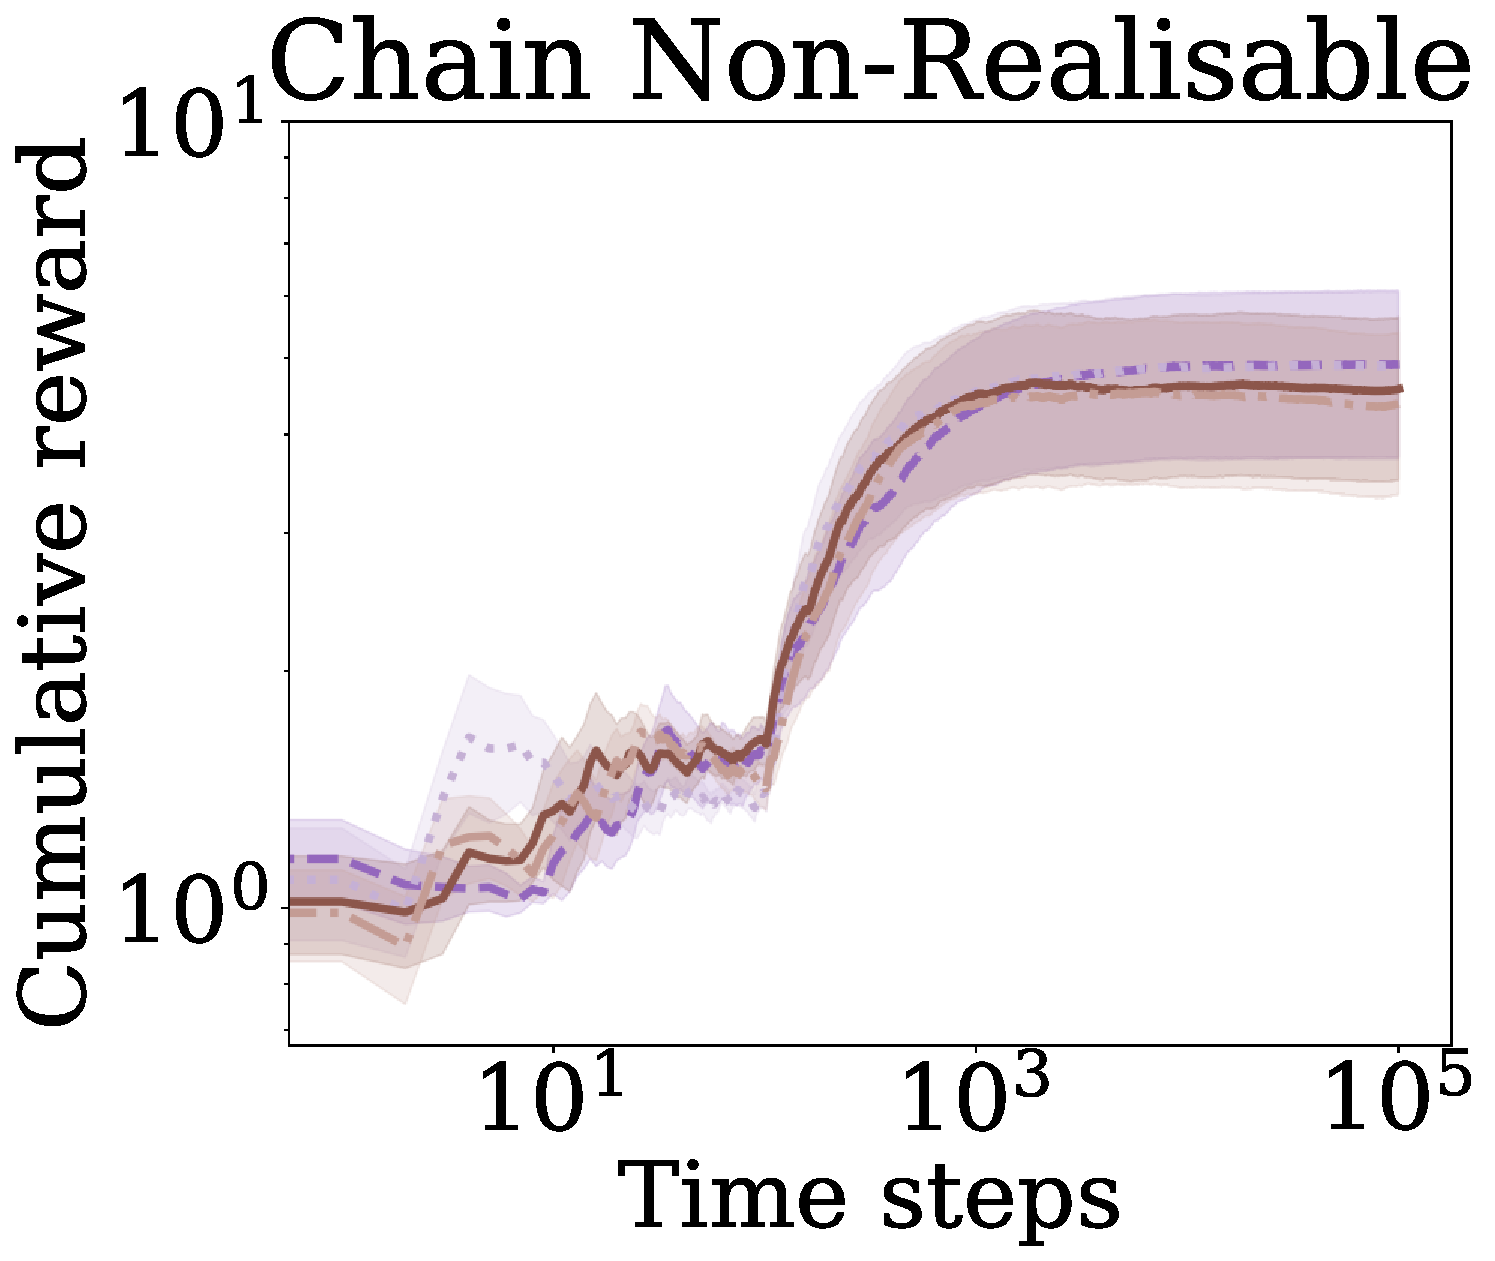
\includegraphics[width=0.35\textwidth]{img/chain_meta_non_realisable.pdf}\\
%     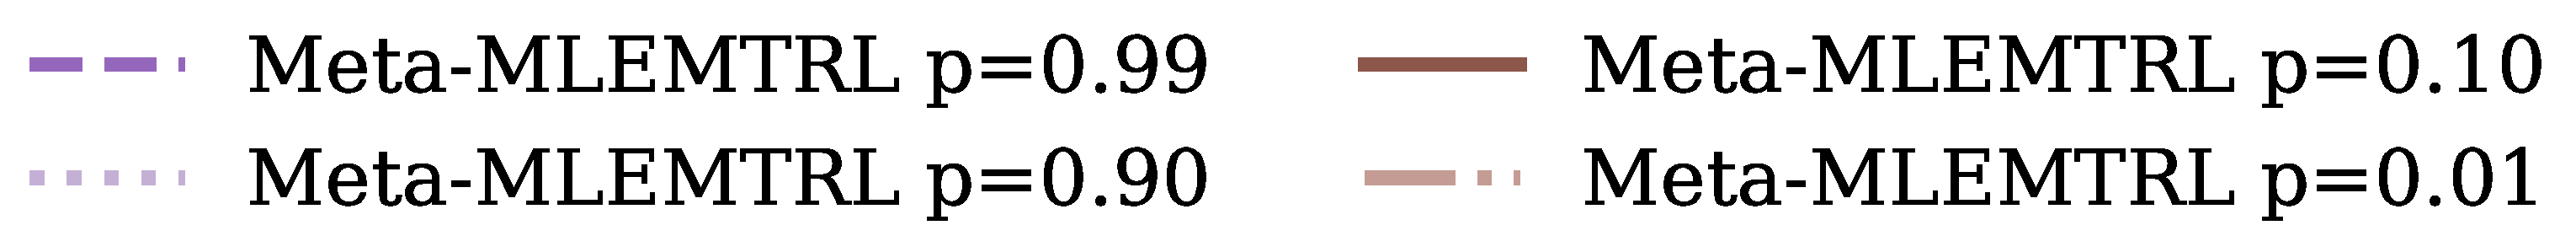
\includegraphics[width=0.96\textwidth]{img/lqr_legend3.pdf}
%     \caption{Figure depicting an ablation study of the prior parameter $p$ in the Meta-MLEMTRL algorithm. The y-axis is the average cumulative reward at each time step computed over $10$ novel tasks and the shaded region represents the standard error. When $p=1$, the algorithm reduces to MLEMTRL and when $p=0$ the algorithm reduces to standard maximum likelihood model estimation.}
%     \label{fig:meta_results}
% \end{figure*}

\clearpage
\section{Additional Experimental Analysis}

\subsection{Experimental Setup}\label{sec:rl_env}
The experiments are deployed in \textsc{Python 3.7}, with support from \textsc{SciPy}~\citep{virtanen2020scipy}, \textsc{Stable-baselines3}~\citep{raffin2021stable} and ran on a i5-4690k CPU and a GTX-960 GPU. The parameters for the variations of SAC and PPO are kept to be the default ones.

\noindent\textbf{RL Environments: Chain.} A common testbed for RL algorithms in tabular settings is the Chain~\citep{dearden1998bayesian} environment. In it, there is a chain of states where the agent can either walk forward or backward. At the end of the chain, there is a state yielding the highest rewards. At every step, there is a chance of the effect of the opposite action occurring. This is denoted as the slipping probability. The slippage parameter is also what is used to create the source models, in this case, those parameters are $\{0.01, 0.20, 0.50\}$. 
For PSRL and MLEMTRL we use a product-NormalGamma prior over the reward functions. For PSRL, we use product-Dirichlet priors over the transition matrix.
%\iffalse
%\begin{figure}[t!]
%    \centering
%    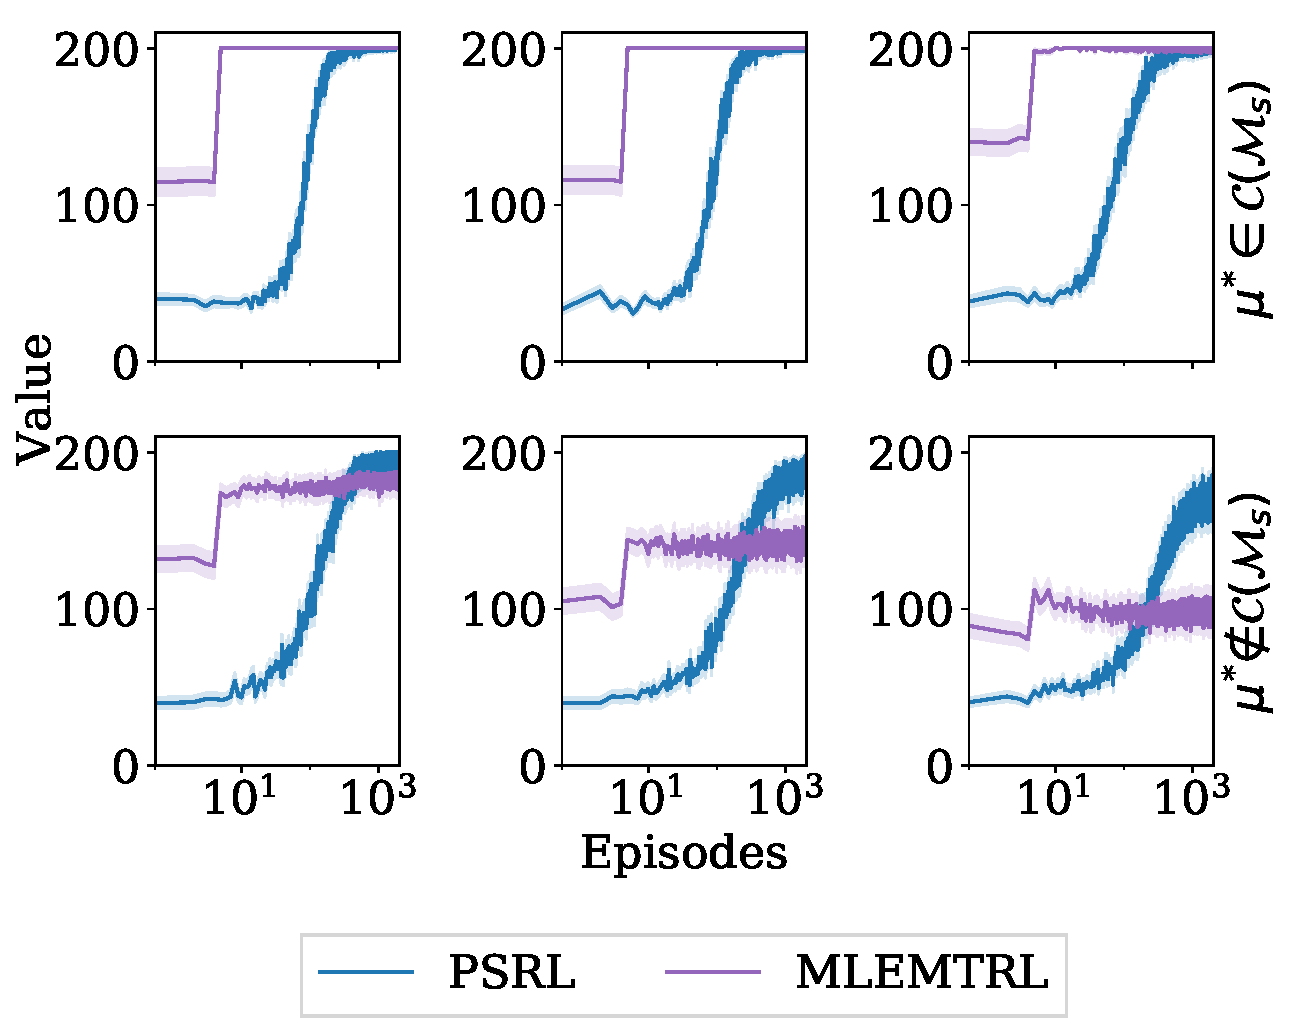
\includegraphics[width=0.5\textwidth]{img/time_experiment.pdf}
%    \caption{We compare MLEMTRL against PSRL in terms of convergence speed and early performance. The value functions of the algorithms are plotted against the log of the number of episodes. The shaded area is the $68\%$ confidence of the mean over multiple MDPs with the same model dissimilarity. In the topmost row, all of the true MDPs are within the convex hull $\mathcal{C}(\mathcal{M}_s)$. In the bottom row, the MDPs are outside. As you go from top-left to bottom-right, the divergence from the true model to the average model in the convex hull increases. For utility, higher values are better.}
%    \label{fig:time}
%\end{figure}
%\fi


%\noindent\textbf{CartPole.}
%The environment used to testbed our algorithm is the \emph{Cartpole} environment~\citep{barto1983neuronlike}. The task is to stabilise a pole attached to a cart and keep it upright for the total episode length of $200$ time steps. The state-space $s \in \mathbb{R}^4$ and the action-space $a \in [-1, 1]$. A continuous action applies a bounded force in the opposite direction on the cart. 
%The original environment parameters are the \emph{gravity} $g=9.8$, \emph{mass of cart} $m=1.0$, \emph{mass of pole} $p=0.1$ and \emph{length of pole} $l = 0.5$. In order to construct our source tasks, we create a variation of these parameters. For more details, see Appendix. 
%\iffalse
%in the following way, \hecomment{this can be in appendix since it confused reviewers}
%\[
%  \mathcal{M}_s = \kbordermatrix{
%    & g & m & p & l \\
%    \mdp_1 & 9.80 & 1.00 & 0.10 & 0.50 \\
%    \mdp_2 & 43.84 & 1.89 & 0.50 & 0.93 \\
%    \mdp_3 & 46.29 & 0.34 & 0.44 & 0.13 \\
%    \mdp_4 & 46.34 & 1.93 & 0.49 & 2.47 \\
%    \mdp_5 & 18.95 & 2.36 & 0.37 & 1.64
%  }.
%\]
%\fi

\noindent\textbf{RL Environments: LQR Tasks.}
We investigate two LQR tasks in the \emph{Deepmind Control Suite}~\citep{tassa2018deepmind}, namely \emph{dm\_LQR\_2\_1} and \emph{dm\_LQR\_6\_2}. These environments are continuous state and actions whereby the task is to control a two joint one actuator and six joint two actuators towards the center of the platform for the two tasks, respectively. They consist of unbounded control inputs and rewards with the state spaces $s \in \mathbb{R}^4$ and $s\in\mathbb{R}^{12}$, respectively. In the Deepmind Control suite every task is made to be different by varying the seed at creation. The seed determines the stiffness of the joints.


\noindent\textbf{RL Environments: CartPole.} We also conduct some experiments on the CartPole~\citep{barto1983neuronlike} environment. In this case, we use a continuous control version of it and formulate it as a LQR problem. The environment has a single continuous action and a state space $s \in \mathbb{R}^4$. To create different tasks we vary the environmental parameters of the problem, namely the gravity, mass of cart, mass of pole the length of the pole.

\subsection{Impacts of Realisability}
In the experiment depicted in Figure~\ref{fig:time}, we investigate the convergence rate and the jumpstart improvement of the MLEMTRL algorithm on $100$ independent target MDP realisations at six different levels of divergence. The divergence is measured from the centroid of the convex hull to the target MDP. Further, in the topmost row, all of the target MDPs belong to the convex hull of source models. 


\begin{figure}[h!]
   \centering
   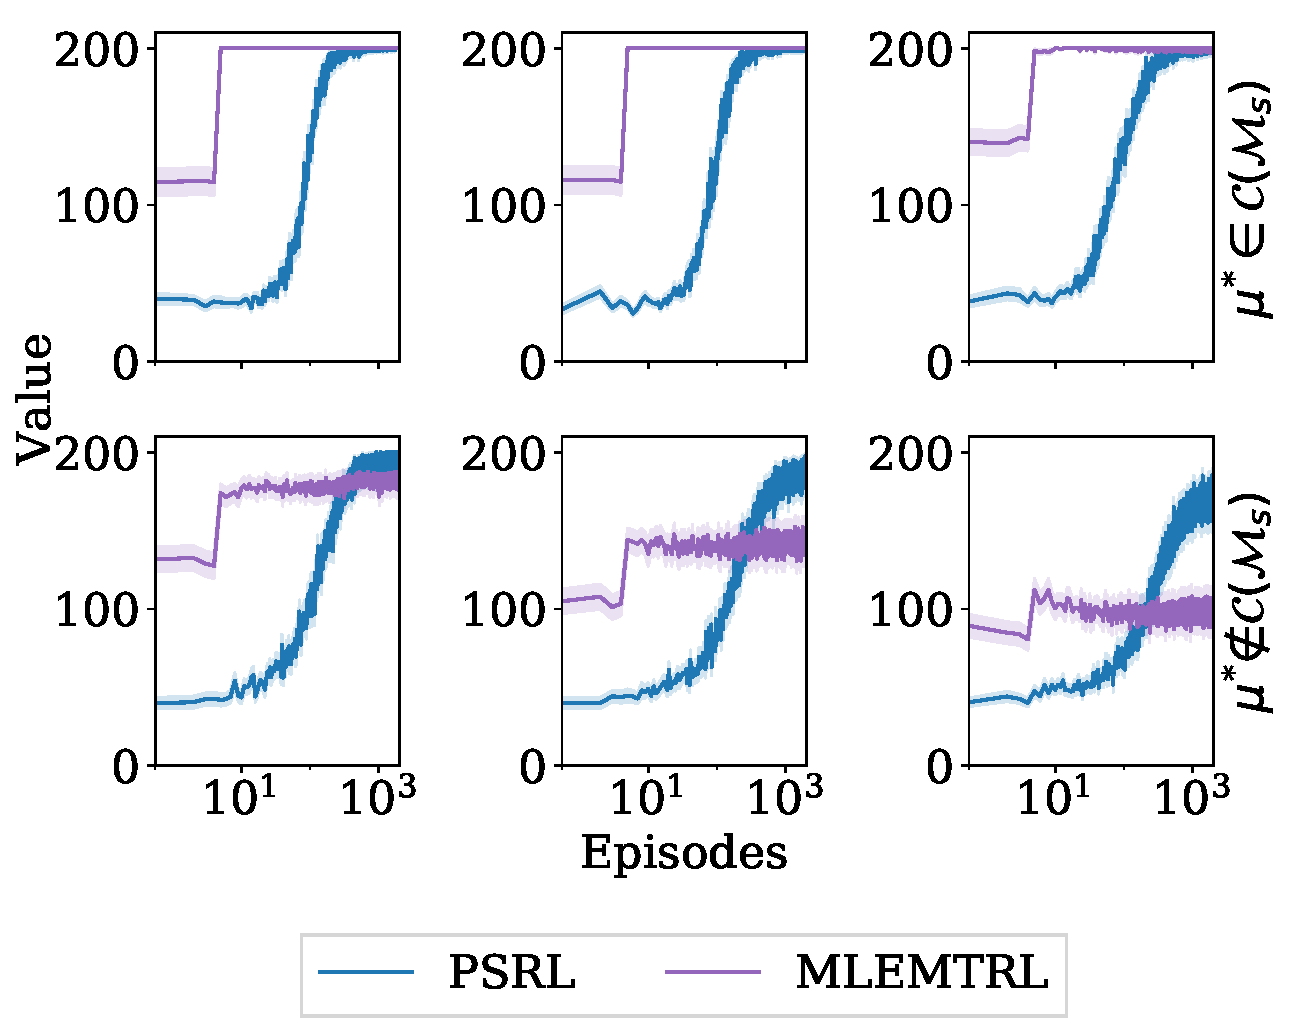
\includegraphics[width=0.55\textwidth]{img/time_experiment.pdf}
   \caption{We compare MLEMTRL against PSRL in terms of convergence speed and early performance. The value functions of the algorithms are plotted against the log of the number of episodes. The shaded area is the $68\%$ confidence of the mean over multiple MDPs with the same model dissimilarity. In the topmost row, all of the true MDPs are within the convex hull $\mathcal{C}(\mathcal{M}_s)$. In the bottom row, the MDPs are outside. As you go from top-left to bottom-right, the divergence from the true model to the average model in the convex hull increases. For utility, higher values are better.}  \label{fig:time}
\end{figure}
As we can see, in this setting, identification of the true model occurs rapidly. One reason for this is because of the near-determinism of the environment. Compared to the agent learning from scratch, we observe zero-regret with faster convergence. As we go from top-left to bottom-right, the divergence increases. For the bottom-most row, we can again observe a faster learning rate. In this case, the degradation in performance increases with the divergence, resulting in poor performance in the final case. The experiment demonstrates that under the TRL framework, we require that the source models are not too dissimilar from the target model.
%These source tasks are then used to transfer knowledge from to the novel task. The maximum attainable return in this environment is $200$ which happens if the agent is able to balance the pole for the full episode length. In this setting, the MLEMTRL algorithm effectively creates a mixture of linear-Gaussians as the full likelihood model and obtains the mixture weights by using experience from the novel task.


\iffalse
\subsection{Full Table Results}
\begin{table*}[t!]
    \centering
    \label{table:full_table}
    \caption{Shown is the standard error of the mean of the average total reward per step (for Chain, and the LQR tasks) and the standard error of the mean of the total return (for the CartPole environment). R/NR signifies whether the novel tasks are realisable or non-realisable by the source tasks.}
    \begin{tabular}{l | c c c c c c c }
        Environment & PSRL & SAC & MT-SAC & MT-SAC-TRL & MT-PPO & MT-PPO-TRL & MLEMTRL \\ \hline
        Chain$_\mathrm{R}$ & & & & &&&\\
        Chain$_{\mathrm{NR}}$ & & & & &&&\\
        CartPole$_\mathrm{R}$ & & & & &&&\\
        CartPole$_{\mathrm{NR}}$ & & & &&&\\
        LQR\_2\_1$_\mathrm{R}$ & $0.99 \pm 0.00$ && $0.89 \pm 0.02 $& $0.98 \pm 0.00 $ &&&\\
        LQR\_2\_1$_{\mathrm{NR}}$ & $0.99 \pm 0.00$&& $0.90\pm0.02$& $0.99 \pm 0.00 $ &&&\\
        LQR\_6\_2$_\mathrm{R}$ & $0.94 \pm 0.00$&& $0.96 \pm 0.00$& $0.99 \pm 0.00$ &&&\\
        LQR\_6\_2$_{\mathrm{NR}}$ & $0.98 \pm 0.00$&& $0.96 \pm0.00 $& $0.98 \pm 0.01 $ &&&
    \end{tabular}
\end{table*}
\fi

\newpage
\subsection{Impacts of Multi-Task Learning as a Baseline}
In Figure~\ref{fig:sac_results} we investigate the performance increase of using multi-task RL and transfer RL compared to regular RL. The baseline algorithm is Soft Actor-Critic and its associated multi-task and transfer learning formulations. As we can see, \textbf{MT-SAC-TRL} appears to have overall strongest performance, with \textbf{MT-SAC} a close second. Because of the nature of the problem (unbounded negative rewards), it is also possible for the algorithms to diverge during learning, which further strengthens the argument for using multi-task or transfer learning for robustness.
\begin{figure*}[h!]
    \centering
    \includegraphics[width=0.4\textwidth]{img/lqr_2_1_sac_realisable.pdf} %\hfill
    \includegraphics[width=0.4\textwidth]{img/lqr_6_2_sac_realisable.pdf}\\
    \includegraphics[width=0.4\textwidth]{img/lqr_2_1_sac_non_realisable.pdf} %\hfill
    \includegraphics[width=0.4\textwidth]{img/lqr_6_2_sac_non_realisable.pdf}\\
    
\includegraphics[width=.5\textwidth]{img/lqr_legend2.pdf}
    \caption{Figure depicting the performance boost of using multi-task and transfer reinforcement learning compared to standard reinforcement learning. The y-axis represents average cumulative reward at every time step and the shaded region is the standard error.}
    \label{fig:sac_results}
\end{figure*}


\newpage
\subsection{Model-based Transfer Reinforcement Learning with Known Reward Function}
In Figure~\ref{fig:known_reward_results}, we aim to contrast the difference from the figure in the main paper where now the reward function is known a priori to \textbf{MLEMTRL} and \textbf{PSRL}.
\begin{figure*}[h!]
    \centering
    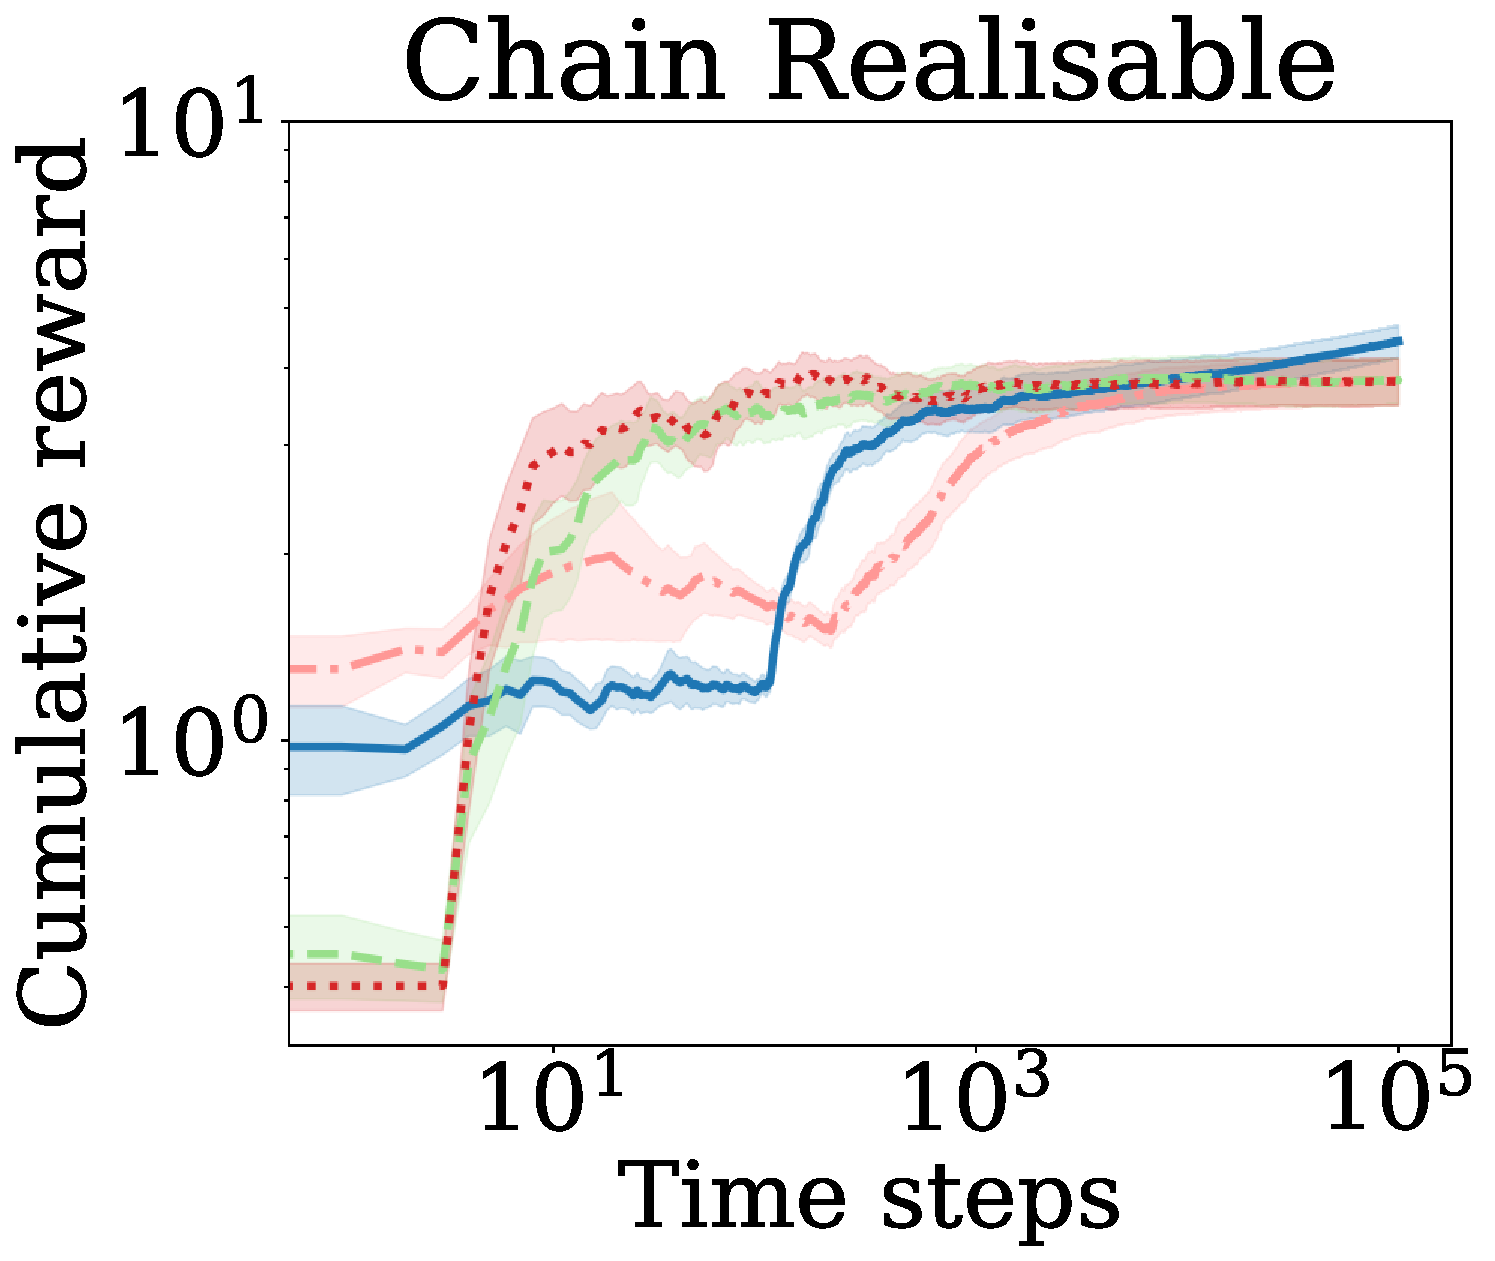
\includegraphics[width=0.4\textwidth]{img/chain_known_realisable.pdf} 
    \includegraphics[width=0.4\textwidth]{img/chain_known_non_realisable.pdf}\\
    
\includegraphics[width=0.96\textwidth]{img/lqr_legend.pdf}
    \caption{Performance of MLEMTRL, the meta algorithms, and the baselines for the case with known reward function in Chain. The y-axis is the average cumulative reward at every time step and the shaded region is the standard error.}\label{fig:known_reward_results}
\end{figure*}